

\subsection{Task 1: source sentence}

A source sentence can be seen as a trivial linear finite-state acceptor whose arcs are labelled with the words in original order. Consider the example \texttt{the black dog}, Figure \ref{fig:src} illustrates one way to encode it as a transducer.

\begin{figure}[h]\centering
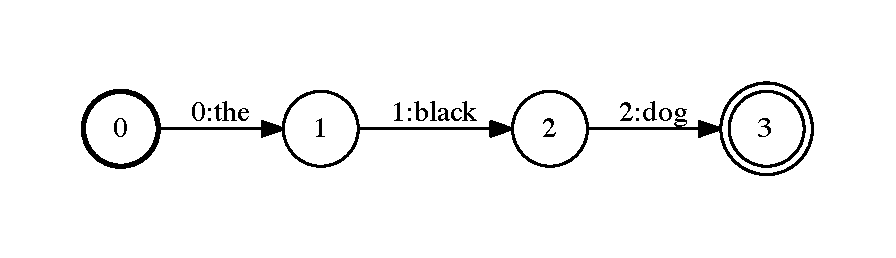
\includegraphics[scale=0.5]{src.pdf}
\caption{\label{fig:src}Input seen as a transducer: the label encodes an input position and its corresponding word.}
\end{figure}

Table \ref{tab:task1} summarises the task. 

\begin{table}[h]\centering
\begin{tabular}{l p{12cm}}
\textsc{Task}   &  encode source sentences as transducers \\
\textsc{Input}  &  first 100 English sentences in \texttt{dev.en} \\
\textsc{Output} &  one transducers for each sentence\\
\textsc{Submit} & nothing to submit here\\
\textsc{Report} & add a graphical illustration for one example from \texttt{dev.en} \\
\end{tabular}
\caption{\label{tab:task1}Task 1 summarised}
\end{table}
